\section{Contexto en RASimAs}
\label{art:rasimas}

El \ac{WP} 3 del proyecto \ac{RASimAs} tiene como objetivo crear \nuevo{un} modelo virtual con anatomía especifica de pacientes. Con el objetivo de conseguir el máximo realismo posible, se propone como objetivo crear modelos virtual que pueda usarse en el simulador que contenga anatomía real de pacientes. Para ello se propone crear la herramienta \ac{TPTVPH}.
Este juego de herramientas está diseñado para permitir crear un \ac{VPH} y que pueda ser posicionado y movido durante su uso en el simulador.

Para lo cual, debido a su complejidad el \ac{WP} se divide en varias tareas.
\begin{itemize}
    \item Tarea 3.1 Adquisición de datos:
        A partir de imágenes de \ac{IRM}, \ac{TC}, etc... se conseguirá un modelo virtual que servirá como entrada para las tareas siguientes.
    \item Tarea 3.2 Modelado anatómico:
        Finalización de los modelos superficiales de los tejidos que se han recuperado de la tarea anterior.
    \item Tarea 3.3 Modelado mecánico:
        El objetivo es conseguir o modelar el comportamiento mecánico de los tejidos como los músculos 
    \item Tarea 3.4 Modelado fisiológico:
        Esta tarea está focalizada en crear el comportamiento de los nervios y el consecuente movimiento de los músculos. 
    \item Tarea 3.5 Integración:
        Con el resultado de todas las tareas anteriores, es posible automatizar y crear una herramienta para que partiendo de las imágenes iniciales pueda crearse un paciente virtual.
    \item Tarea 3.6 Posicionamiento de pacientes:
        Por último, es necesario modificar la posición del paciente a la posición requerida por \ac{RA}. 
\end{itemize}

\begin{figure}[h]
   \centering
    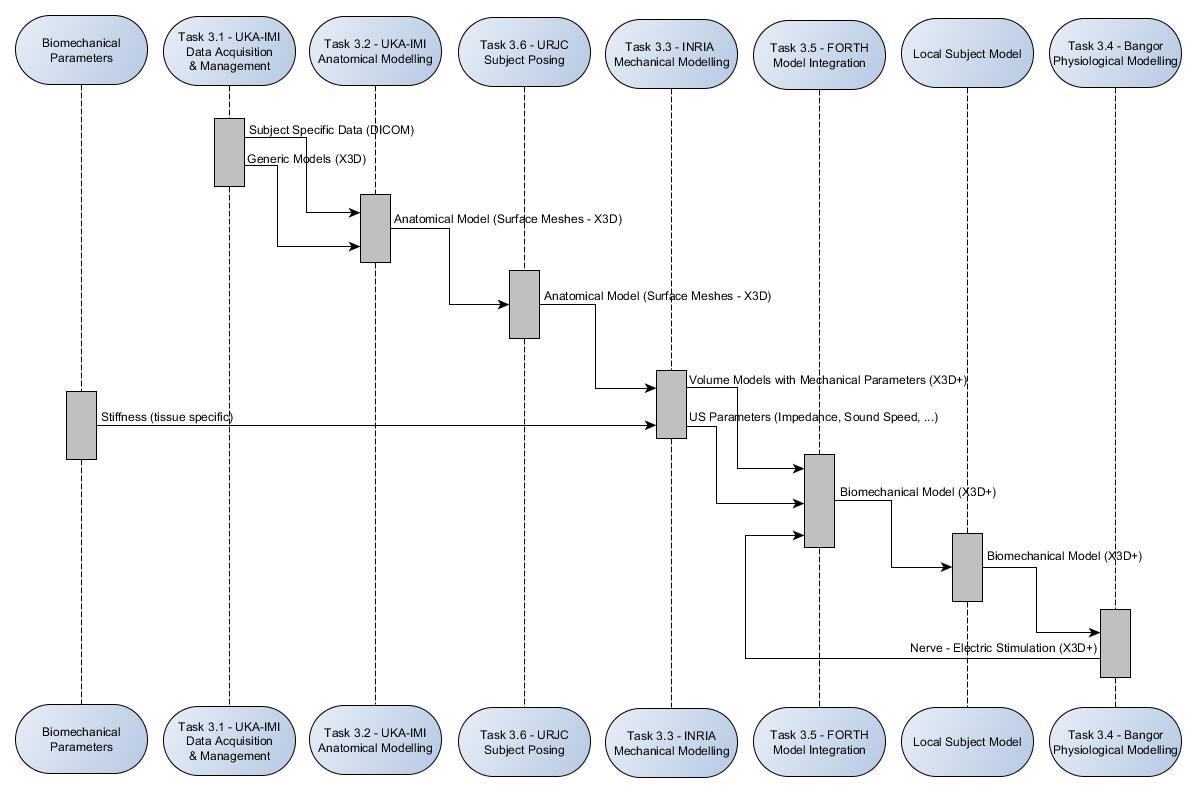
\includegraphics[width=0.5\textwidth]{IMG/RASimAs_D3.png}
    \caption{ }
   \label{fig:WP3}
\end{figure}


Por tanto, la tarea 3.6 necesita crear un método que sea capaz de modificar la posición de un paciente virtual a su posición final, de manera que pueda usar todos o varios resultados intermedios de las tareas anteriores a esta. Como parte de ese trabajo, esta tesis presenta una solución que se centra en resolver de manera innovadora los problemas encontrados.

\todo{meter wp 5?}
